% sections/appendices.tex
\clearpage
\pagenumbering{arabic} % if you want arabic numbers in the appendices

\begin{appendices}

\chapter{Supplementary material}

\section{Structural setup}
\label{app:ciso}
\begin{figure}[htbp]
  \centering
  % scale to the full text width, keep aspect ratio
  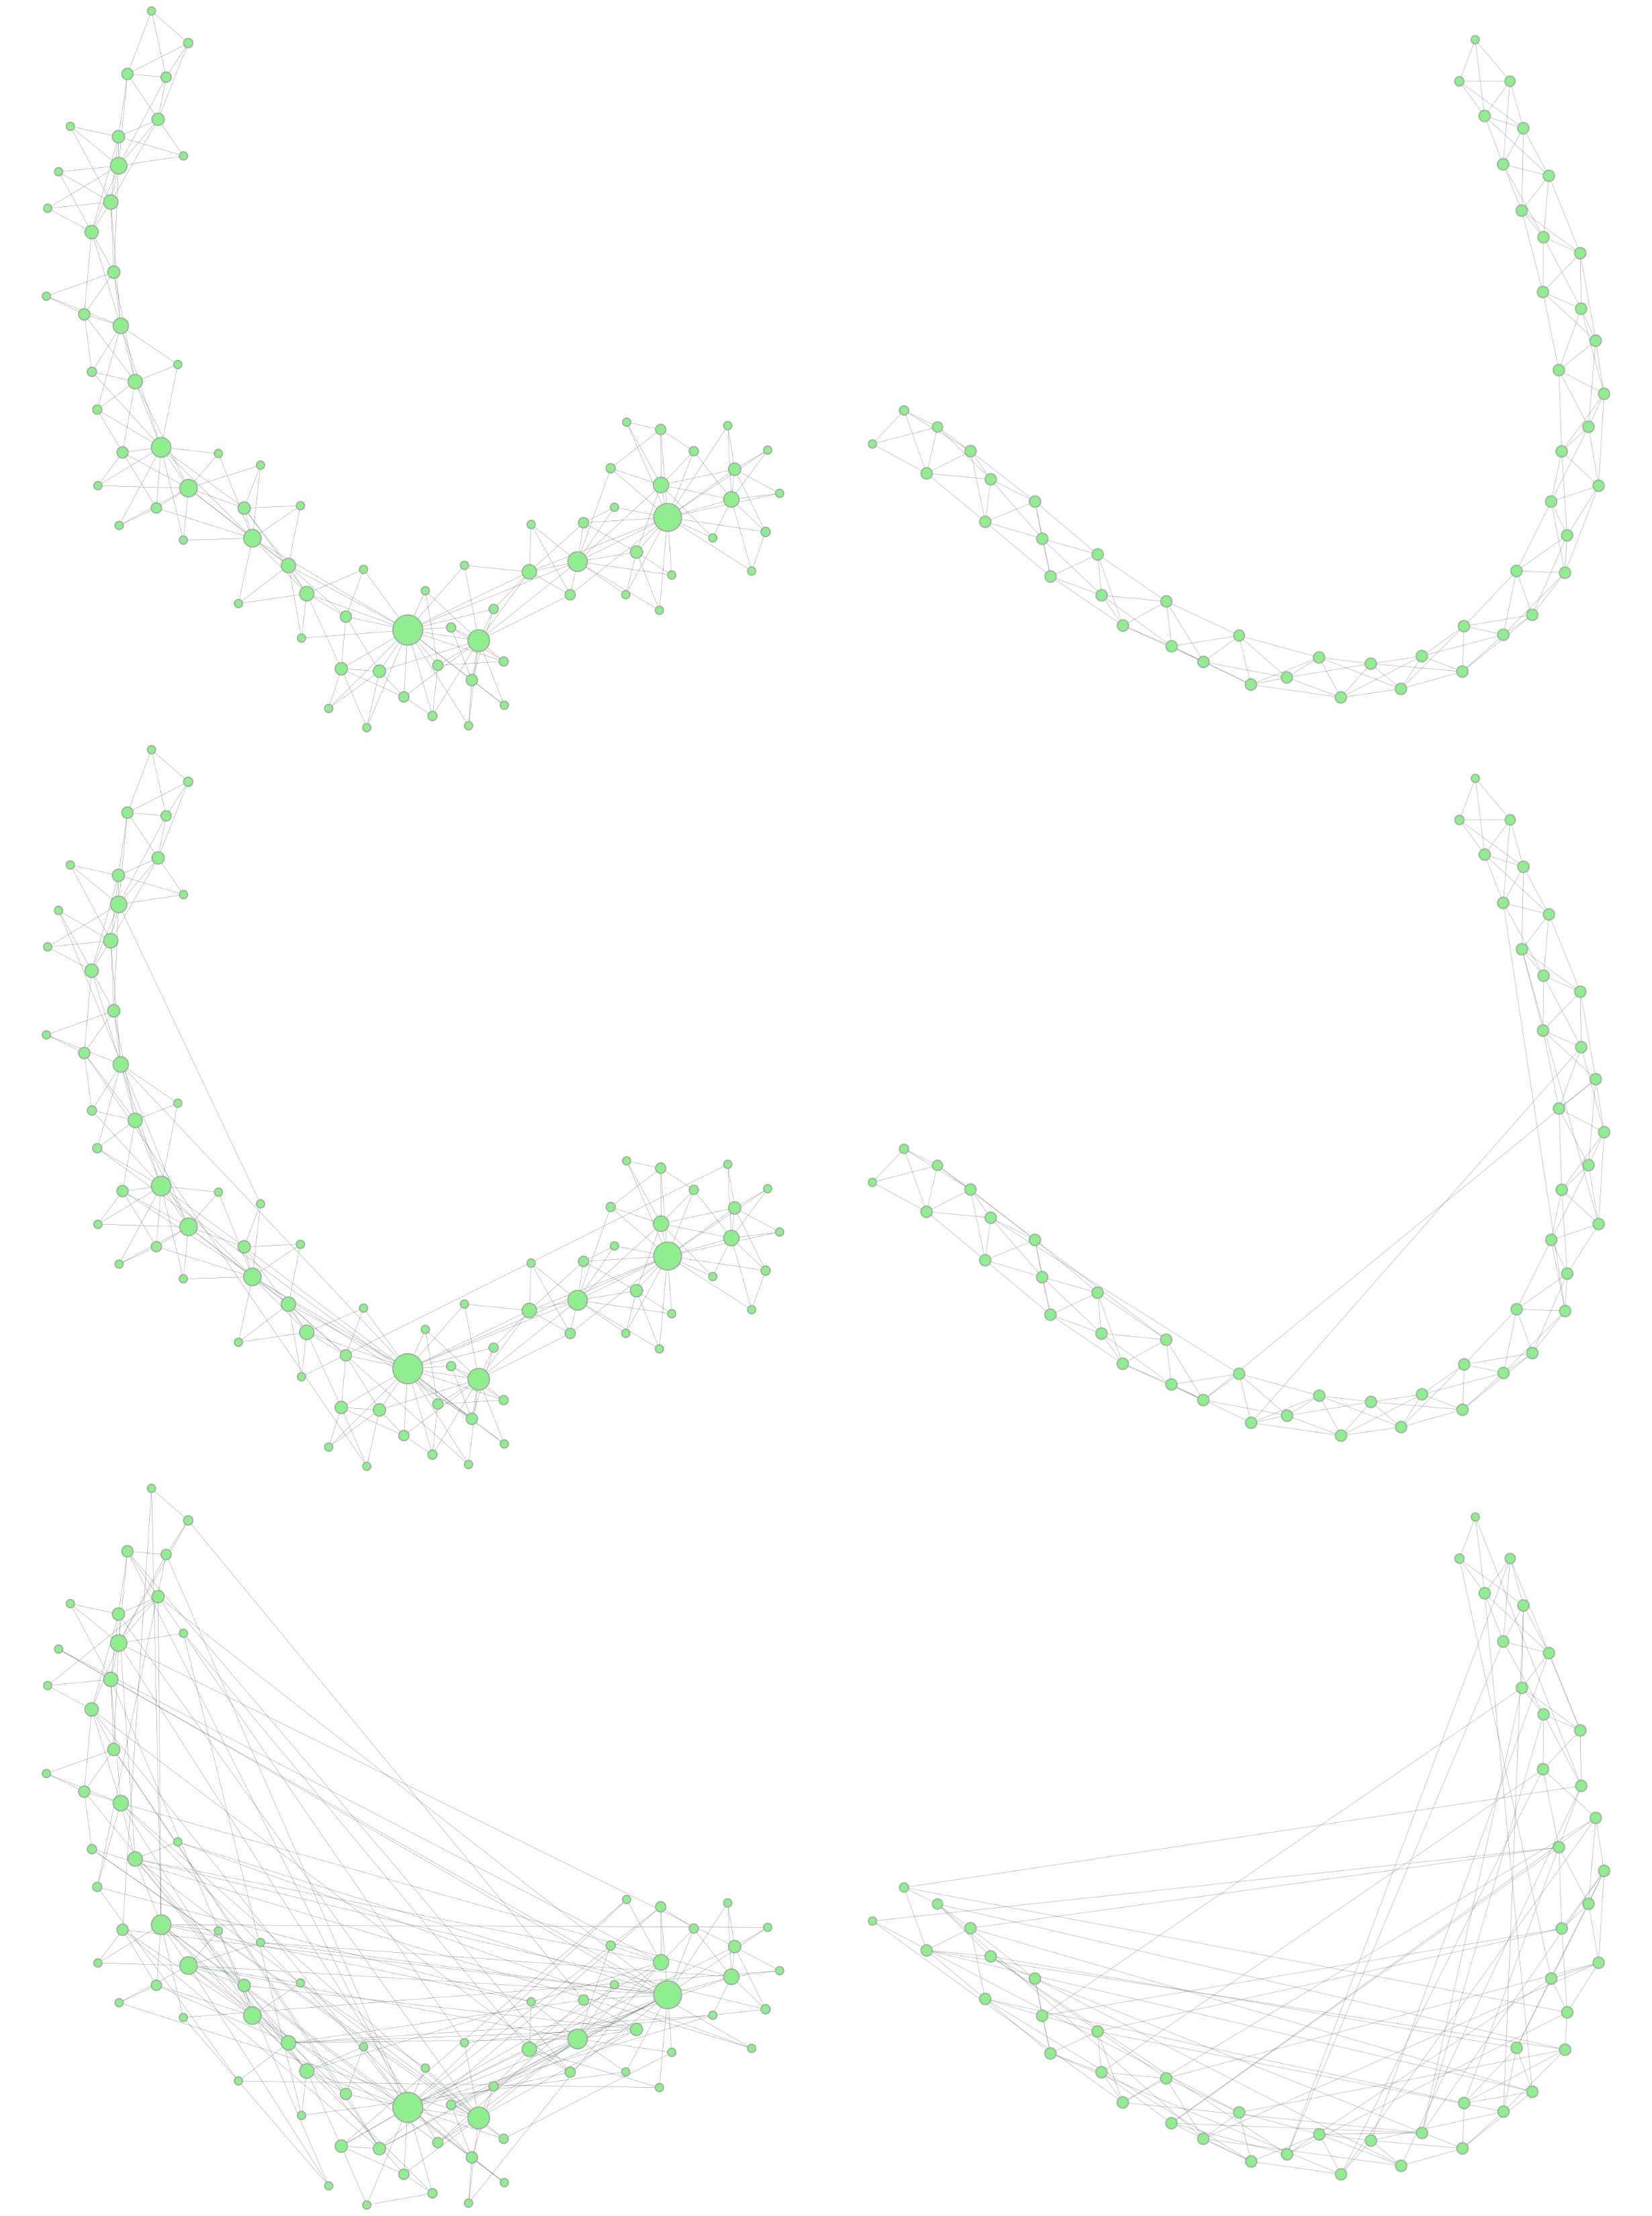
\includegraphics[width=10.5cm,keepaspectratio]{images/SWSF_Vs_SW.jpg}
  \caption{At the top there is a structured scale free and a regular lattice, both 1-dimensional, then a rewiring procedure is employed, constructing a so called small world scale free (SWSF) and a small world network, for a value of the rewiring parameter p = 1 we have a scale free random graph on the left and a homogeneous random graph on the right, }
  \label{fig:yourlabel}
\end{figure}

\section{Noise investigation and other}

\begin{figure}[htbp]
  \centering
  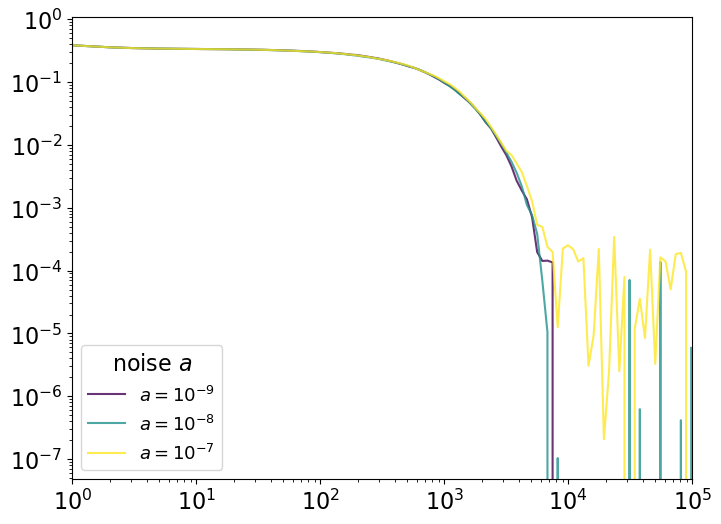
\includegraphics[width=14cm,keepaspectratio]{images/BA_low_noise.png}
  \caption{Investigation of the behavior of low noise experiments on a BA network with m=2, the temporal variance is even larger, and the middle noise is characterized by spikes,they could be reflection of the transient between states in the unimodal phase, but is not a good guess}
  
\end{figure}
\begin{figure}[htbp]
  \centering
  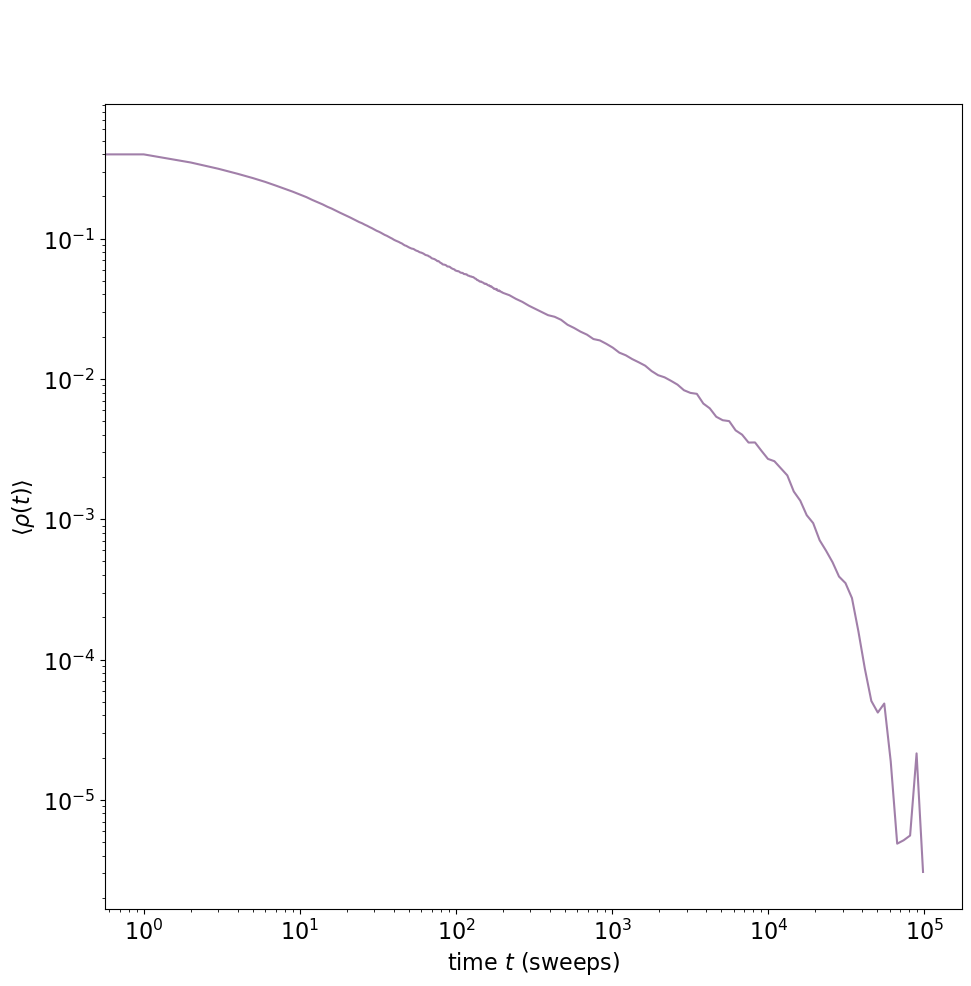
\includegraphics[width=9cm,keepaspectratio]{images/quick_check.png}
  \caption{run on a SSF network wirh $N=1000$ to verify that finite size exponential decay indeed kicks in later as declared in the main section}
  
\end{figure}
\begin{figure}[htbp]
  \centering
  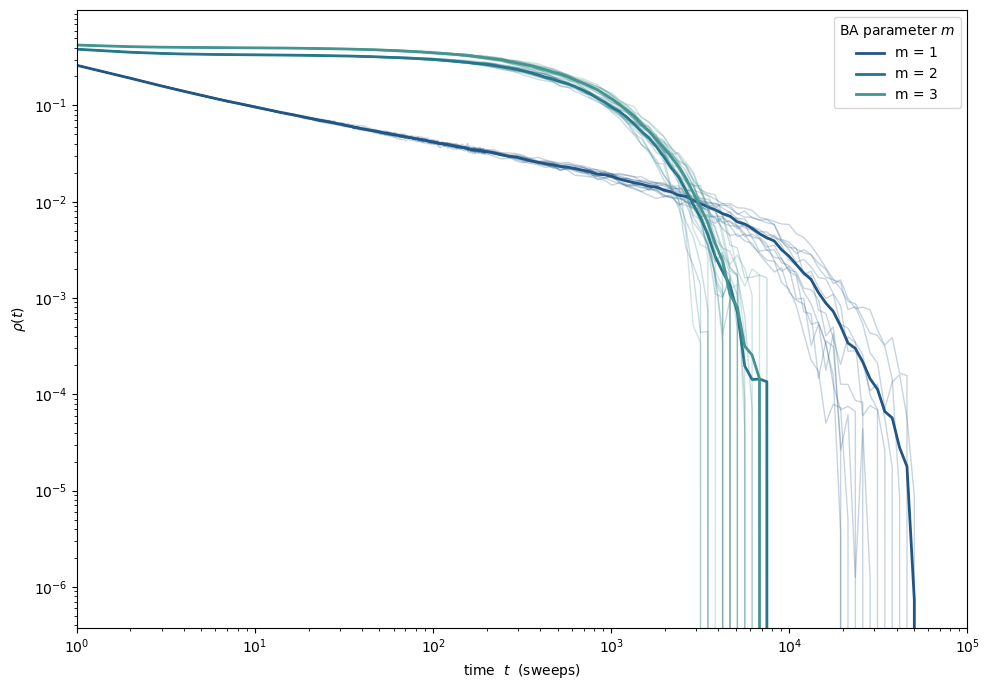
\includegraphics[width=14cm,keepaspectratio]{images/BA_classic.png}
  \caption{Classic voter model on BA networks at increasing values of m, the light trajectories are the 12 single-graph trajectories of which the main ones are the average, when a plateau exists (m>1), its value is an increasing function of m.}
  
\end{figure}


\chapter{Some remarks}
\section{Voter model}
It would be interesting to address quantitatively both the plateau value and the the lifetime of the system, for the former, single runs must be analyzed, because the plateau represents a metastable state for the system and has a precise value per graph realization; in theory it should be affected by quenched disorder, but maybe the effects vanish in the termodinamic limit.\\
Looking at  \ref{fig:vm comparison}, a perplexing phenomena is also the difference in behaviour between the SSF and the BA ($m=1$), the only thing they share is having a spectral dimension smaller than two, but its curious how the BA seems to be a lower bound for the SSF, being just tangent to it right before the decay, this is also true for the 1d lattice, other low dimansional topologies should be studied to see how they relate with each other.\\

Finally, the authors of \cite{suchecki2005voter} never mention the spectral dimension, but they don't define clearly what dimension are they talking about, they talk about disorder (parameter $p$) wich can be understood to be small-worldness, and dimension separately, it would be interesting to compare the voter model dynamics while keeping in mind the three concepts of average path length, topological, and spectral dimension, finding the edge cases could confirm or refute that the spectral dimension is truly the only deciding factor for determining if the system will order or not. 
\section{European rail network}
The easiest way to address Y-junctions is to simply add metadata based on angles, some kind of node variable that tells a walker:"if you come from $a$ you cannot go to $b$" (as in \ref{fig: junctionexample}) so that the distance $d(a,b) = d(a,c) + d(b,c)$; "purer" approaches failed: I couldn't find a directed subgraph to replace the junction node with and achieve desired effect, nor is effective the idea to transform from $G$ to $L(G)$ delete there, and then anti-transform (the anti-transorfm doesn't exist once you remove the desired nodes).
For degree-4 nodes, I found it almost impossible to tell if the rails are simply crossing or there is an actual junction, angles don't always cut it.\\ 
Another thing that I saw was that stations, especially bigger ones, tend to have clumps of $ns$ nodes around them, in reality big stations are far from being points, rather, they extend over a (possibly vast) area. A simple strategy could be just to delete all nodes close to a station and give it all their connections, although defining a universal radius is not straightforward.\\
\end{appendices}
